\documentclass[xcolor={usenames,svgnames,x11names,dvipsnames,table}]{beamer}

\usetheme{SBUclass}

\usepackage{mypackages}
\usepackage{mycommands}

\title{\texorpdfstring{Language \& Technology}{Language and Technology}}
\subtitle{Wrapping Up}
\author{Al{\"e}na Aks{\"e}nova \& Aniello De Santo}
\institute{Stony Brook University\\\texttt{alena.aksenova@stonybrook.edu}\\\texttt{aniello.desanto@stonybrook.edu}}
\date{}


\begin{document}
\unnumbered{
\begin{frame}
	\titlepage
\end{frame}
}

\begin{frame}{TL;DR --- Be Skeptical}
    \begin{itemize}
            \item Technological advances can bring much good but...\\
        \item Humans overestimate technology.\\
            \subpoint{Loebner Prize\slash Turing test}
        \item Don't buy the hype.\\
            \subpoint{deep learning, artificial intelligence, culturomics, neuroscientism, \ldots}
        \item Technological advances also come with downsides.\\
            \subpoint{social biases, rising job requirements, mass surveillance, \ldots}
    \end{itemize}
\end{frame}

\begin{frame}{The State-of-the-Art in Language Technology} 
    \begin{itemize}
        \item Current technologies often involve \highlight{n-grams models}.
            %
            \begin{itemize}
                \item word completion\slash prediction
                \item stylistic analysis
                \item OCR
                \item spell checking
                \item web search
                \item word meaning
                \item machine translation
            \end{itemize}
        \item Frequency information from corpora\slash tree banks is used to\\
            add \highlight{probabilities} to the models.
            \pause
          \item Caveat: in this class we have (mostly) ignored most modern trends\\
          $\Rightarrow$ Neural Networks and Deep Learning
    \end{itemize}
\end{frame}



\begin{frame}{Language is Complex}
    \begin{itemize}
        \item Language comes easy to humans,\\
            but it is \highlight{incredibly complex}.
            \begin{itemize}
                \item culture-specific rules of turn taking
                \item building sentence meaning from word meaning
                \item tons of variation across languages and dialects
              \item hidden structure of sentences
                \item how that hidden structure is inferred
            \end{itemize}
        \item We have to deal with this complexity.
        \item Probabilities won't cut it because of \highlight{Zipf's law}.
                    \item (Psycho)Linguistic insights will help us evaluate/improve existing technologies.
    \end{itemize}
\end{frame}


\begin{frame}{Why There is no Hope for bare N-Gram Models}
    $n$-grams can only consider local information, but\\
    language often uses \highlight{non-local information}.

    \begin{example}
        \begin{itemize}
            \item Suppose the user is typing \emph{May I of} on their phone.
            \item Do we suggest \emph{off} or \emph{offer} as the best word completion?
            \item \textbf{Bigram Frequencies}\\
                \begin{tabular}{lr}
                    I offer & \highlight{0.00014\%}\\
                    I off   & 0.00001\%
                \end{tabular}
            \item But what if the user had typed \emph{May I quickly of}?
            \item \textbf{Bigram Frequencies}\\
                \begin{tabular}{ll}
                    quickly offer & 0.00000025\%\\
                    quickly off   & \highlight{0.000002\%}
                \end{tabular}
        \end{itemize}
    \end{example}
\end{frame}

\begin{frame}{Scaling Up Doesn't Help}
    \begin{itemize}
        \item Okay, so bigrams don't work, but trigrams would:\\
            \emph{I quickly offer} is more frequent than \emph{I quickly off}
        \item But what if the user had typed

            \begin{center}
                \begin{tabular}{rr}
                    May I really quickly of & 4-grams!\\
                    May I really really quickly of & 5-grams!\\
                    $\vdots$
                \end{tabular}
            \end{center}
        \item This isn't feasible, we quickly run into \highlight{data sparsity issues}.
    \end{itemize}
\end{frame}

\begin{frame}{Non-Local Dependencies}
    \begin{itemize}
        \item Dependencies in language aren't limited to a fixed number $n$ of words, they can span arbitrary distances:
            \begin{itemize}
                \item \emph{The man that I think Bill thinks I think \ldots Bill punched seems angry.}
                \item \emph{The men that I think Bill thinks I think \ldots Bill punched seem angry.}
            \end{itemize}
    \end{itemize}
    %
    \begin{block}{The Linguistic Moral of the Story}
        \begin{itemize}
            \item $n$-gram models will never work perfectly,\\ not even if we had unlimited resources.
            \item \textbf{Reason:} Linguistic dependencies can be unbounded and thus\\ span over
                more than $n$ words.
        \end{itemize}
    \end{block}
\end{frame}

\begin{frame}{How Complex are Sentences?}
    \begin{itemize}
        \item We have seen that \highlight{$n$-gram models are insufficient}.
        \item But what should we use instead?
    \end{itemize}
\end{frame}

\begin{frame}{Sentences Have Hidden Structure}
    \begin{itemize}
        \item Linguists have known for a long time that sentences are not just sequences of words.
        \item They involve a lot of hidden structure $\Rightarrow$ \highlight{trees!}
    \end{itemize}
    %
    \begin{center}
        \begin{forest}
            [S, for tree={parent anchor=south, child anchor=north}
                [NP
                    [N [Cats] ]
                ]
                [VP
                    [V [bite] ]
                    [NP
                        [N [dogs] ]
                    ]
                ]
            ]
        \end{forest}
    \end{center}
\end{frame}

\begin{frame}{Some Evidence for Hidden Structure}
    \begin{itemize}
        \item Some but not all strings of words can be moved around.
    \end{itemize}
    %
    \begin{exe}
        \ex
        \begin{xlist}
            \ex[] {It is \colored{teal}{old ugly dogs} that cats bite \colored{teal}{\_\_}.}
            \ex[*] {It is \colored{teal}{dogs} that cats bite \colored{teal}{old ugly \_\_}.}
        \end{xlist}
    \end{exe}
    %
    \begin{itemize}
        \item Some but not all strings can be coordinated.
    \end{itemize}
    %
    \begin{exe}
        \ex
        \begin{xlist}
            \ex[] {Cats \colored{teal}{bite old ugly dogs} and \colored{purple}{scratch young cute dogs}.}
            \ex[*] {Cats \colored{teal}{bite old ugly} and \colored{purple}{scratch young cute} dogs.}
        \end{xlist}
    \end{exe}
    %
    \begin{itemize}
        \item Verbal agreement is not determined by closest noun.
    \end{itemize}
    %
    \begin{exe}
        \ex
        \begin{xlist}
            \ex[] {The woman is tired.}
            \ex[] {The women are tired.}
            \ex[*] {The women that buried the woman is tired.}
            \ex[] {The women that buried the woman are tired.}
        \end{xlist}
    \end{exe}
\end{frame}

\begin{frame}{Even More Evidence for Hidden Structure}
    \begin{itemize}
        \item Questions front the \highlight{structurally highest auxiliary},\\
            not the first one in the string.
    \end{itemize}
    %
    \begin{exe}
        \ex
        \begin{xlist}
            \ex[] {The man who \colored{teal}{is} looking for a job \colored{purple}{is} exasperated.}
            \ex[*] {\colored{teal}{Is} the man who \colored{teal}{\_\_} looking for a job \colored{purple}{is} exasperated?}
            \ex[] {\colored{purple}{Is} the man who \colored{teal}{is} looking for a job \colored{purple}{\_\_} exasperated?}
        \end{xlist}
    \end{exe}
    %
    \begin{itemize}
        \item lots of evidence from experiments\\
            \subpoint{self-paced reading, eye tracking, ERP, fMRI}
    \end{itemize}
%
%    \begin{followup}
%        \begin{columns}
%            \column{.75\linewidth}
%            \begin{itemize}
%                \item Lin 311 \emph{Syntax}
%                \item Richard Larson's \emph{Grammar as Science}
%                \item my lecture notes (added to Blackboard)
%            \end{itemize}
%
%            \column{.25\linewidth}
%            \quad
%            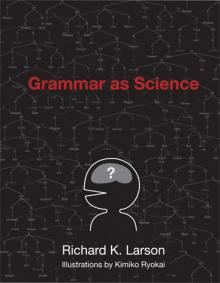
\includegraphics[height=5em]{./img/grammarasscience}
%            \quad
%            \phantom{a}
%        \end{columns}
%    \end{followup}
\end{frame}


\begin{frame}{Related Linguistics Courses}
    \begin{itemize}
        \item LIN 101 \emph{Human Language}\\
        \item LIN 110 \emph{Anatomy of English Words}\\
        \item LIN 200 \emph{Language in the USA (online!)}\\
        \item as background for sentence models:\\
            LIN 311 \emph{Syntax}\\
            LIN 346 \emph{Language \& Meaning}\\
             LIN 347 \emph{Pragmatics}\\
        \item as background for speech recognition:\\
            LIN 201 \emph{Phonetics}\\
            LIN 301 \emph{Phonology}
    \end{itemize}

    \pause
    \begin{block}{Possible Courses Spring 2020 (taught by yours truly)}
        \begin{itemize}
            \item LIN 425 \emph{Computational Psycholinguistics}
            \item LIN 260  \emph{Language \& Mind}
        \end{itemize}
    \end{block}
\end{frame}

\begin{frame}{Computational-oriented Faculty in Linguistics}

    \begin{center}
           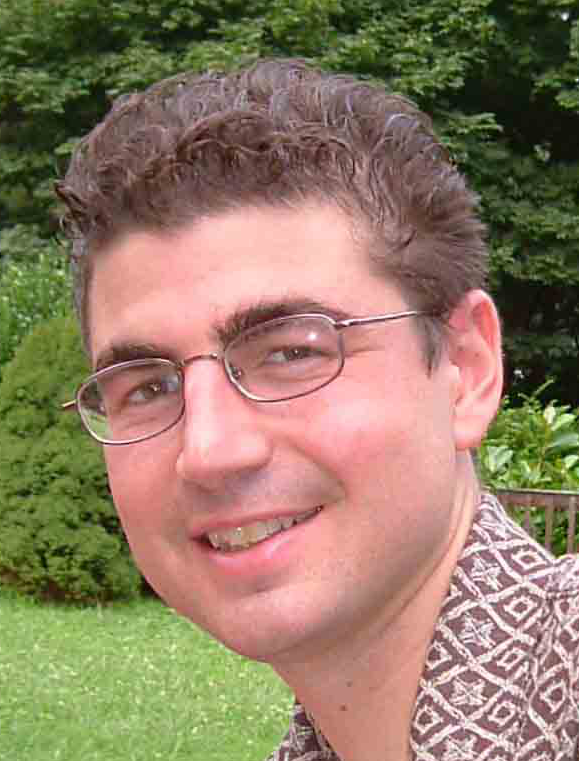
\includegraphics[height=5em]{./img/heinz_crop}
        \hspace{4em}
         
\includegraphics[height=5em]{./img/thomas_graf}
            \hspace{4em}
            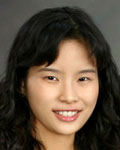
\includegraphics[height=5em]{./img/jiwon_yun}\\
                \noindent
        \footnotesize\bfseries
                \href{http://jeffreyheinz.net}{Jeff Heinz}  \hspace{4em} \href{http://thomasgraf.net}{Thomas Graf}  \hspace{4em} \href{https://linguistics.stonybrook.edu/jiwonyun/index.html}{Jiwon Yun} \\          
    \end{center}
   
  \pause
  \vspace{1cm}
  \begin{center} 
   \alert{\textbf{\href{http://compling.stonybrook.edu/}{Check out our lab and brand new M.A. Program.}}}
    \end{center}
\end{frame}

\begin{frame}{Computational Opportunities in Linguistics}
    \begin{enumerate}
            \item \textbf{LIN 488 UG Teaching Practicum (Fall 2019)}\\
            Be a UG TA for LIN 120! \alert{If interested, shoot me an email by the end of May.}
             \emph{Prerequisite}: A decent grade in this class.
        \item \textbf{LIN 488 Internship (Fall 2019)}\\
           I might need research assistants for my dissertation project. Get in touch if interested.\\
            \emph{Prerequisite}: LIN 311 Syntax, or talk to me.
        \item \textbf{LIN 628 - Computational Syntax (Fall 2019)}\\
            Mathematical models of sentence structure (it's a grad class).\\
            \emph{Prerequisite}: LIN 311 Syntax, or talk to Thomas Graf.
                    \item \textbf{LIN 220 Computational Linguistics (Spring 2020)}\\
            A follow up to this class. Taught by me.
    \end{enumerate}
\end{frame}


\begin{frame}{Two Course Recommendations Outside Linguistics}
    \begin{enumerate}
        \item SOC 330 \emph{Media and Society}\\
            (Jason J.~Jones; no programming, but a bit of computational sociology and big data)
        \item AMS 103 \emph{Applied Math in Technology}\\
            (Matthew Reuter; includes a live cookie baking session)
    \end{enumerate}
\end{frame}

\begin{frame}{Programming Concepts}
    \begin{itemize}
        \item \textbf{Universal}
            \begin{itemize}
                \item strings, integers, lists
                \item variables
                \item print, input
                \item conditionals
                \item while loops
                \item for loops
                \item custom functions
                \item regular expressions
            \end{itemize}
        \item \textbf{Python-Specific}
            \begin{itemize}
                \item counters
                \item positions and slices
                \item built-in functions like \texttt{len}, \texttt{str.lower}, \ldots
            \end{itemize}
    \end{itemize}
\end{frame}

\begin{frame}{Sticking with Python}
    \begin{itemize}
        \item You invested lots of time and energy on picking up some programming skills.
              They \highlight{should not go to waste}!
        \item The most important thing: find yourself a \highlight{project}!
    \end{itemize}

    \begin{block}{Project suggestions}
        \begin{itemize}
            \item Computational analysis in a book report
            \item Automatic menu generator for New York hipster restaurants
            \item Facebook bot to like all your friends' posts and\\
                  leave a short reply
            \item Script to delete all unread emails that are older than 30 days
            \item Reminder to take a break after 2h in front of the screen
            \item Automating something you frequently do manually
        \end{itemize}
    \end{block}
\end{frame}

\begin{frame}{Some Project Ideas from Reddit}
    Check out the \href{https://www.reddit.com/r/Python/comments/308ucq/how_do_you_use_python_to_automate_tasks_in_life/}{Reddit thread}:

    \medskip
    \pause
    \begin{quote}
        Our department keeps a calendar of activities in excel.
        I use python to import that spreadsheet, break the activities into itemized tasks, put due dates on each task, and spit out those tasks for each teammate.
    \end{quote}

    \pause
    \begin{quote}
        I stitched together a video encoding script, a mp3 tag reading script and a YouTube uploading script to automatically upload all of the old music I'd recorded to YouTube. Saved me 100s of hours of manual work. 
    \end{quote}
\end{frame}

\begin{frame}{Some Project Ideas from Reddit [cont.]}
    \begin{quote}
        This is a pretty silly usage, but the autopy package is really great for making auto-clickers for various web-games. 
    \end{quote}

    \begin{quote}
        I have a script that checks the Powerball and Megamillions jackpot size and calculates the expectation value of a play. If either is positive, it sends me a text to buy a ticket.
    \end{quote}

    \begin{quote}
        Not complete yet, but I am using python on a RasPi to automate the temperature, humidity, and lighting for my two pythons' cages
    \end{quote}
\end{frame}


\begin{frame}{Other Fun Stuff with Python}
    \begin{itemize}
        \item Python coding for \emph{Minecraft}\\
            \href{http://www.instructables.com/id/Python-coding-for-Minecraft/}{http://www.instructables.com/id/Python-coding-for-Minecraft/}
        \item Modding \emph{The Sims 4}\\
            \href{http://simswiki.info/wiki.php?title=Tutorials:TS4_General_Modding}{http://simswiki.info/wiki.php?title=Tutorials:TS4\_General\_Modding}
        \item Creating hi-res texture mods (e.g.\ for Resident Evil 4 HD)\\
            \href{https://youtu.be/u_8I3vaVrfE}{https://youtu.be/u\_8I3vaVrfE}
        \item \emph{Gray Hat Python} book on hacking with Python
    \end{itemize}
\end{frame}

\begin{frame}{Code Combat \& Code Wars}
    \centering

    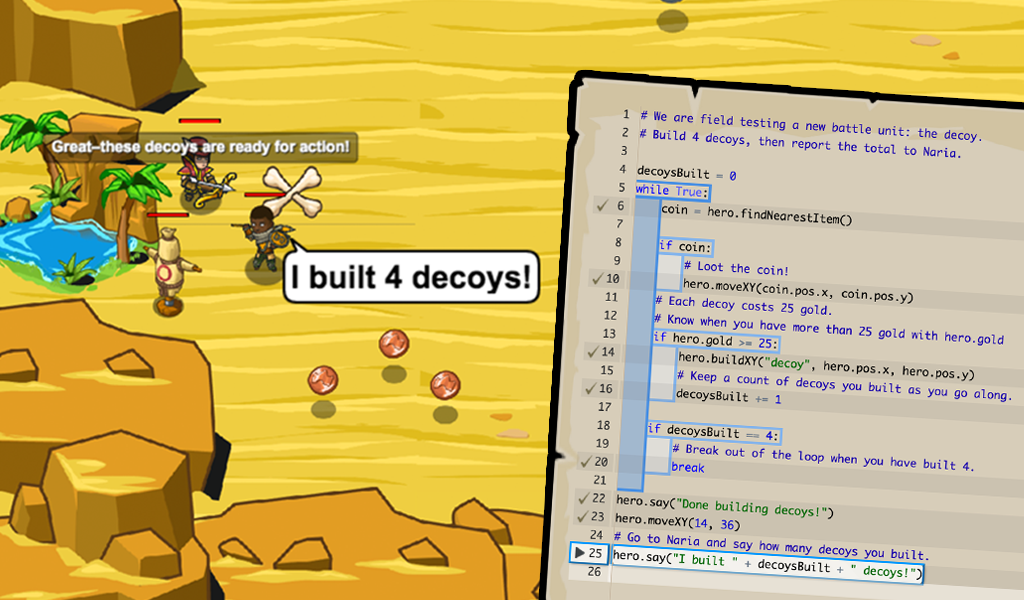
\includegraphics[width=.8\linewidth]{./img/codecombat}

    If you liked Code Combat, check out \href{https://www.codewars.com/}{Code Wars}!
\end{frame}

\begin{frame}{How much Python Do I Know?}
    \begin{itemize}
        \item We covered enough Python for 90\% of all problems.
        \item But Python can do a lot more:
            \begin{itemize}
                \item strides
                \item dictionaries (of which Counters are a special case)
                \item unpacking
                \item zipping
                \item recursive functions
                \item object oriented programming with classes
                \item generators
                \item decorators
            \end{itemize}
        \item And there's many powerful libraries:
            \begin{itemize}
                \item pyplot
                \item pandas
                \item ntlk
                \item scipy
                \item scikit-learn
            \end{itemize}
        \item Don't worry about any of this for now.
    \end{itemize}
\end{frame}

\begin{frame}{Additional Teaching Materials}
    If at some point you need to know more Python for your project,
    check out some of these:

    \begin{itemize}
        \item The remainder of our textbook\\
                \emph{Automate the Boring Stuff With Python}
        \item The programming historian\\
            \href{http://programminghistorian.org/}{http://programminghistorian.org/}
        \item Python programming for the humanities\\
            \href{http://www.karsdorp.io/python-course/}{http://www.karsdorp.io/python-course/}
        \item Natural language processing with Python\\
            \href{http://www.nltk.org/book/}{http://www.nltk.org/book/}
        \item Mark Summerfield's book \emph{Programming in Python 3}
        \item For more theory, check out the book \emph{Language and Computers}
    \end{itemize}
\end{frame}

\begin{frame}{Don't do it Alone!}
    \begin{itemize}
        \item Form learning\slash reading groups with your classmates.
        \item Check out SBU undergraduate clubs and the events they host.
        \item Join online communities.
        \item Need advice?
            Send me an email or come to my office hours!
    \end{itemize}
\end{frame}

\begin{frame}{The End (?)}
    \begin{center}
           
\includegraphics[width =  \textwidth]{./img/maxresdefault}
        \end{center}
\end{frame}

\end{document}
